\documentclass[twoside,10pt,a4paper]{article}
\usepackage[utf8]{inputenc}
\usepackage[english]{babel}
\usepackage{amsmath}
\usepackage{amsfonts}
\usepackage{amssymb}
\usepackage{graphicx}

\usepackage[left=2cm,right=2cm,top=2cm,bottom=3cm]{geometry}
\usepackage{fancyvrb}
\usepackage{listings}
\usepackage{xparse}
\usepackage{tikz} % ajout de dessins LaTeX
\usepackage{graphicx}
\usepackage{float}  % alignement des figures
\usepackage{fancyhdr}
\usepackage{enumitem}
\usepackage{verbatim}
\usepackage{xcolor}
\usepackage{cancel}

\usepackage{caption}
\usepackage{subcaption}

\pagestyle{fancy} %fancyhdr
	\fancyhf{} %fancyhdr
	\renewcommand{\sectionmark}[1]{\markboth{#1}{}}
	\fancyhead[R]{NLDCI Set 7 Questions} %INSERT TITLE HERE FOR fancyhdr
	\fancyhead[L]{\nouppercase{\leftmark}} %fancyhdr
	\cfoot{\thepage} %fancyhdr
	\setlength{\headheight}{35pt}
	\setlength{\parindent}{0pt}
	
	\definecolor{MyBlue}{HTML}{4A90E2}
	\definecolor{MyRed}{HTML}{D0021B}
	\definecolor{MyGreen}{HTML}{7ED321} % Same color use in Mathcha

\begin{titlepage}
\title{\huge \textbf{Nonlinear Dynamics \& Chaos I \\ \Large Exercice Set 7 Questions}}	%TITLE
\author{ }		%AUTHOR
\date{ }	%DATE

\end{titlepage}


\begin{document}

\maketitle

\section*{Question 1}
Consider a planar Hamiltonian system
\begin{align*}
	\dot{x} &= \frac{\partial H(x,y)}{\partial y} + f_1(x,y), \\
	\dot{y} &= - \frac{\partial H(x,y)}{\partial x} + f_2(x,y),
\end{align*}
where the twice continuously differentiable function $H(x,y)$ is the Hamiltonian associated with the system (say, the energy in classical mechanics, or the stream function in fluid mechanics), and the continuously differentiable $\mathbf{f} = (f_1, f_2)$ is a dissipative term (say, damping in classical mechanics, or compressible terms in fluid mechanics). Assume that $\nabla \cdot \mathbf{f} \neq 0$ for all $(x,y) \in \mathbb{R}^2$. (Linear damping, for instance has this property.)

Show that the above system can have no limit cycles.

\section*{Question 2 - Accuracy of averaging}
Show that on time scales of $\mathcal{O}(1/\varepsilon)$, a solution $\mathbf{x}(t)$ with $\mathbf{x}(0) = \mathbf{x}_0$ of the dynamical system
\begin{equation}\label{Q01E01}
	\dot{\mathbf{x}} = \varepsilon \mathbf{f}(\mathbf{x},t, \varepsilon), \qquad \mathbf{x} \in \mathbb{R}^n,
\end{equation}
($\varepsilon$ is a small parameter and $\mathbf{f}$ is a smooth function that is $T$-periodic in time) remains $\mathcal{O}(\varepsilon)$-close to any solution $\mathbf{y}(t)$ with $\mathbf{y}(0) = \mathbf{x}_0 + \mathcal{O}(\varepsilon)$ of the averaged system
\begin{equation}\label{Q01E02}
	\dot{\mathbf{y}} = \varepsilon \bar{\mathbf{f}}_0 (\mathbf{y}), \qquad \mathbf{y} \in \mathbb{R}^n,
\end{equation}
where
\begin{equation*}
	\bar{\mathbf{f}}_0 (\mathbf{y}) = \frac{1}{T} \int_0^T f(y,t,0) \, \text{d}t.
\end{equation*}
\textit{Hint}: Subtract (\ref{Q01E02}) from (\ref{Q01E01}) and integrate to obtain an expression for $|\mathbf{x}(t) - \mathbf{y}(t)|$. Estimate $|\mathbf{x}(t) - \mathbf{y}(t)|$ from above using the facts that $\bar{\mathbf{f}}$ is Lipschitz and $|\hat{f} - \bar{f}|/\varepsilon$ is uniformly bounded, where $\hat{f}$ is the right-hand-side of the system into which (\ref{Q01E01}) is transformed by the averaging transformation $\mathbf{x} = \mathbf{y} + \varepsilon \mathbf{w}(\mathbf{y},t)$. Then use the following generalized Gronwall inequality:

If $u(t), v(t), c(t)$ are non-negative functions, $c(t)$ is differentiable, and
\begin{equation*}
	v(t) \leq c(t) + \int_0^t u(s)v(s) \, \text{d}s,
\end{equation*}
then
\begin{equation*}
	v(t) \leq c(0) e^{\int_0^t u(s)\, \text{d}s} + \int_0^t c'(s)e^{\int_s^t u(\tau)\,\text{d}\tau}\, \text{d}s.
\end{equation*}

\section*{Question 3 - Unsteady separation in time-periodic fluid flows}
Fluid trajectories $\mathbf{x}(t) = (x(t),y(t))$ in a two-dimensional time-periodic flow satisfy the differential equations
\begin{equation}\label{Q03E01}
	\begin{aligned}
		\dot{x} &= u(x,y,t), \qquad u(x,y,t) = u(x,y,t+T), \\
		\dot{y} &= v(x,y,t), \qquad v(x,y,t) = v(x,y,t+T),
	\end{aligned}
\end{equation}
where $T>0$ is the period, $u$ and $v$ are smooth velocity components satisfying the incompressibility condition $u_x + v_y \equiv 0$. Assume that the fluid is bounded by a wall at $y=0$, on which the velocity field satisfies the no-slip boundary conditions $u(x,0,t) = v(x,0,t)=0$. As a result, all boundary points are nonhyperbolic fixed points for (\ref{Q03E01}).

We say that a boundary point $\mathbf{p}_0 = (x_0,0)$ is a separation point for the flow (\ref{Q03E01}) if $\mathbf{p}_0$ admits an unstable manifold $W^u(\mathbf{p}_0)$. Physically, $W^u(\mathbf{p}_0)$ is a time-dependent curve of fluid particles that shrinks to $\mathbf{p}_0$ is backward time. In forward time, $W^u(\mathbf{p}_0)$ attracts fluid particles, then ejects them from the vicinity of the wall (see Fig. 1). Show that separation points satisfy the criteria
\begin{equation*}
	\int_0^T u_y(x_0,0,t) \, \text{d}t = 0, \quad \int_0^T v_{yy}(x_0,0,t)\, \text{d}t > 0,
\end{equation*}
i.e., separation takes place where the average of the wall-shear is zero and the average of $v_{yy}$ is positive.

\textit{Hint}: Use incompressibility and the boundary conditions to show that (\ref{Q03E01}) can be rewritten as
\begin{align*}
	\dot{x} &= yU(x,y,t), \\
	\dot{y} &= y^2V(x,y,t).
\end{align*}
To focus on the vicinity of the boundary, introduce the scaled variable $y=\varepsilon \eta$, where $0 \leq \varepsilon \ll 1$. Show that the resulting $(\dot{x},\dot{\eta})$ equations are slowly varying and find the corresponding averaged equations. For the averaged equations, rescale time on trajectories by letting $\frac{d\tau}{dt} = \eta(t)$ in order to remove the common $\eta$ factor from the right-hand-side, and look for a hyperbolic fixed point with an unstable manifold off the wall. Use the averaging theorem to relate your results to the original system (\ref{Q03E01}).

\begin{figure}[H]
	\centering
	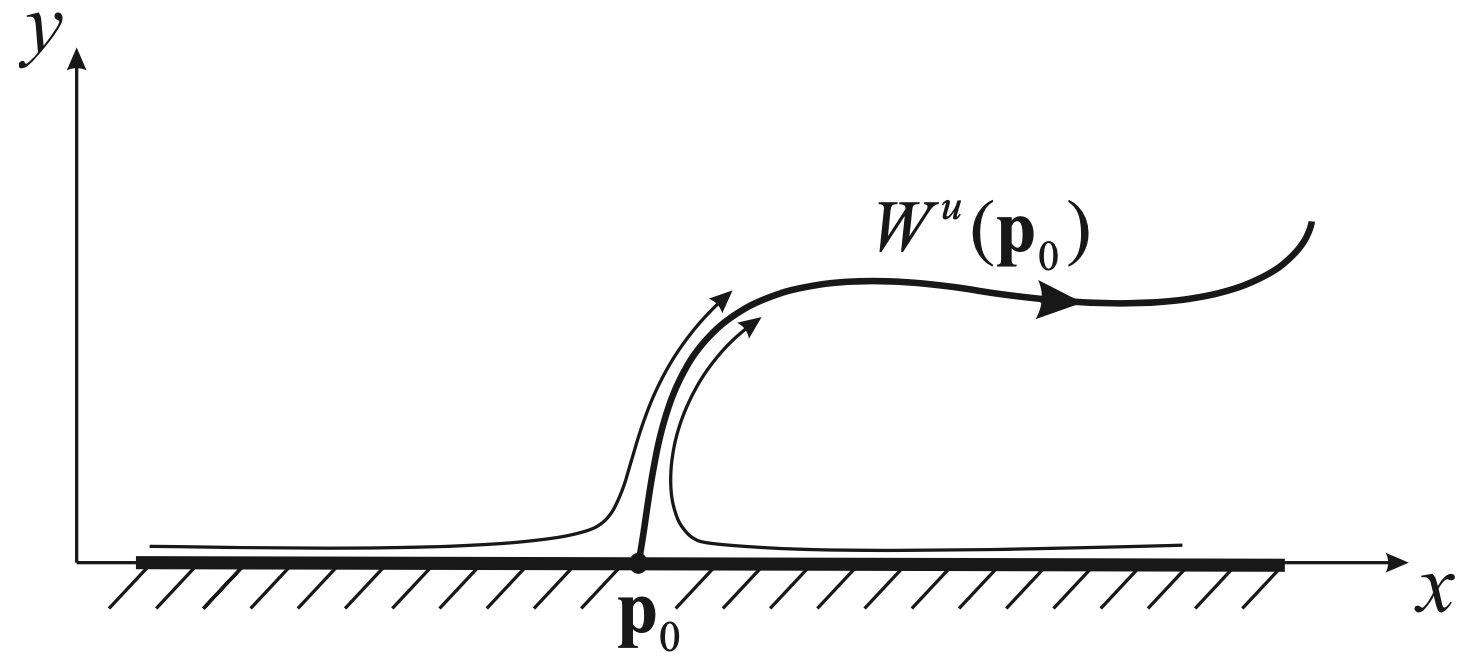
\includegraphics[scale=0.15]{Graphics/Q03D01.png}
	\caption{Unsteady separation from a no-slip wall}
\end{figure}

\section*{Question 4}
Consider the 1D equation
\begin{equation*}
	\dot{x} = \varepsilon (-x + \sin^2(t) + \varepsilon \cos^2(t))
\end{equation*}
Using averaging, determine which statement is correct.

\begin{enumerate}[label=(\alph*)]
	\item $x = 0$ is an attracting fixed point.
	\item $\displaystyle x = \frac{1}{2}$ is an attracting fixed point.
	\item There exists an attracting periodic orbit close to $\displaystyle x = \frac{1}{2}$.
\end{enumerate}

\section*{Question 5}
Which system can be treated by averaging ? Assume that $0 < \varepsilon \ll 1$.

\begin{enumerate}[label=(\alph*)]
	\item $ \ddot{x} + 4x = \varepsilon(1 + x e^t) $
	\item $ \displaystyle \begin{cases}
		\dot{x} = \varepsilon y \sin(t) \\
		\dot{y} = x \cos(\sqrt{2}t)
	\end{cases} $
	\item $ \displaystyle \begin{cases}
		\dot{x} = \varepsilon x^4 \\
		\dot{y} = \varepsilon(x + \sin^2(t))
	\end{cases} $
	\item None of the above
\end{enumerate}

\section*{Question 6}
Consider the dynamical system $ \dot{x} = A(t)x $ with
\begin{equation*}
	A(t) = {\renewcommand*{\arraystretch}{1.25}\begin{pmatrix}
		\displaystyle -1 + \frac{3}{2}\cos^2(t) & \displaystyle 1 - \frac{3}{2} \sin(t)\cos(t) \\
		\displaystyle -1 - \frac{3}{2} \sin(t)\cos(t) & \displaystyle -1 + \frac{3}{2} \sin^2(t)
	\end{pmatrix}}
\end{equation*}
Which of the following statements is correct?

\begin{enumerate}[label=(\alph*)]
	\item The eigenvalues of $A(t)$ are $\displaystyle \lambda_{1,2} = \frac{1}{4}(-1 \pm i\sqrt{7})$. Therefore the $x = 0$ fixed point is stable.
	\item The eigenvalues of $A(t)$ are $\displaystyle \lambda_{1,2} = \frac{1}{4}(-1 \pm i\sqrt{7})$. Therefore the $x = 0$ fixed point is asymptotically stable.
	\item The eigenvalues of $A(t)$ are $\displaystyle \lambda_{1,2} = \pm \frac{i}{2}\cos(2t)$. Therefore the stability of the $x = 0$ cannot be determined.
	\item None of the above
\end{enumerate}

\section*{Question 7}
Does the classic theory of averaging apply to the dynamical system given below?
\begin{equation*}
	\ddot{x} = \varepsilon f(x,t), \quad f(x, t + T) = f(x,t), \quad x \in \mathbb{R}^n
\end{equation*}

\begin{enumerate}[label=(\alph*)]
	\item Yes, after the introduction of the new variable $y = \dot{x}$.
	\item Yes, but only for $ 0 \leq |\varepsilon| \ll 1 $.
	\item Yes, but only for $n = 1$.
	\item None of the above
\end{enumerate}

\section*{Question 8}
Consider the gradient dynamical system:
\begin{equation*}
	\dot{x} = -\nabla V(x)
\end{equation*}
Where $V: \mathbb{R}^n \longrightarrow \mathbb{R}, \; V \in C^1, \; n \geq 2$. Which of the following statements are true?

\begin{enumerate}[label=(\alph*)]
	\item This system cannot have a limit cycle in a region where $\Delta V$ has constant sign.
	\item This system cannot have a limit cycle, because $ V(x(t)) $ is monotone decreasing in $t$.
	\item The system can only have stable limit cycles because of the negative sign in front of $\nabla V(x)$.
	\item None of the above
\end{enumerate}




\end{document}